\documentclass{article}
\usepackage{iclr2027_conference,times}

\usepackage{booktabs}
\usepackage{graphicx}
\usepackage{amsmath}
\usepackage{hyperref}
\usepackage{url}

% ANONYMITY: \iclrfinalcopy must stay commented out for submission -- with it active the
% style file typesets the author block below and the paper is desk rejected. Uncomment BOTH
% it and the \author block for the camera-ready. paper/preflight.py gates this.
% \iclrfinalcopy

\title{Change-Detection Benchmarks for Object-Centric \\ World Models Are Degenerate}

% \author{... restored at camera-ready; the style file substitutes the anonymous block ...}

\begin{document}
\maketitle

\begin{abstract}
Object-centric world models are routinely credited with predicting \emph{which} objects in a
scene will change. We show that the benchmarks used to support that claim are degenerate, and
that the degeneracy is not fixable by filtering the data.
We audit three successive change-detection benchmarks on a tabletop manipulation task, each
constructed to remove its predecessor's shortcut, plus a fourth built to attack the mechanism
we identify, using a battery of eleven rules that have no learned parameters or one.
Every filter does what it was built to do and none of them helps. The motion-filtered
benchmark is won by a one-parameter rule combining velocity and proximity (F1 $0.927$); the
onset filter destroys the velocity term (velocity alone falls $0.866 \rightarrow 0.182$) and
the benchmark is then won by proximity, including a \emph{zero-parameter} rule that predicts
change for the single object nearest the actuator ($0.928$); an interaction filter destroys
proximity in turn ($0.928 \rightarrow 0.437$) and is won by propagated kinematics ($0.955$).
Across all three the best rule in the battery stays between $0.93$ and $0.96$.
Densely packing the scene---the one manipulation that leaves several objects nearly equidistant
from the actuator---does finally lower that ceiling, to $0.821$; but it lowers the learned gate
further, to $0.425$, opening the widest margin in the study. Harder is not the same as
discriminative.
Five published object-centric world models---GNS/DPI-Net, C-SWM, SlotFormer, PETS and
NPS---implemented from their papers, trained with their native objectives and capacity-matched,
lose to these rules on every benchmark, and are degenerate in a second sense: every one flags
essentially all objects as changing (recall $0.993$--$1.000$).
We give the mechanism---with a single actuator and local contact the label is recoverable from
one scalar, and a filter only chooses which---and release the audit battery, together with the
methodological requirement that it be run with rules invented \emph{against} the benchmark
under test rather than against the one it replaces.
\end{abstract}

% =====================================================================================
\section{Introduction}

A recurring claim in object-centric world modelling is that decomposing a scene into objects
lets a model predict \emph{which} objects will be affected by an action, rather than
regressing the whole scene indiscriminately. The claim is intuitive, it motivates a large
family of architectures \citep{battaglia2016interaction,chang2017npe,kipf2020cswm,wu2023slotformer,goyal2021nps},
and it is normally supported by showing that a structured model beats an unstructured one at
change detection on a manipulation benchmark.

The check that is not run is the trivial one. Before concluding that a model has learned which
objects will move, one should ask what a rule with no learned parameters achieves on the same
split. This is standard practice in fields that have been burned: hypothesis-only baselines in
natural language inference \citep{poliak2018hypothesis,gururangan2018artifacts}, question-only
baselines in visual question answering \citep{agrawal2018vqacp,goyal2017vqav2}, and
passage-free baselines in reading comprehension \citep{kaushik2018reading} each showed that a
benchmark's headline numbers were largely recoverable without the input the task was ostensibly
about. We run the equivalent check here, and it fails.

We audit three change-detection benchmarks on a single-actuator manipulation task. They
form a sequence: each was built specifically to remove the shortcut that the audit found in its
predecessor. A fourth, described in Section~\ref{sec:three}, attacks the mechanism rather than
the symptom. Against each we run a battery of eleven rules with zero or one parameter,
including five rules written \emph{before} the third benchmark existed, precisely so that the
audit could not be accused of testing only what the filter was designed to defeat.

The result is that every filter works and none of them helps. Each successive benchmark
demonstrably destroys the rule that won the previous one---velocity falls from $0.866$ to
$0.182$ under the onset filter, and geometry from $0.928$ to $0.437$ under the interaction
filter---while the best rule in the battery stays between $0.93$ and $0.96$ throughout, far
above any learned model we or the literature can put against it. A fourth benchmark, built by
packing the scene so that proximity is genuinely ambiguous, is the one that finally lowers the
ceiling---and lowers the learned models further still, which is the more instructive half of
the finding. Five published
object-centric models, implemented from their papers and capacity-matched, lose to these rules
on every benchmark; all five are degenerate in the stronger sense that they flag essentially
every object as changing.

Our contributions are:

\begin{enumerate}
\item \textbf{A degeneracy result across four benchmarks, four physics engines and five
published models} (Sections~\ref{sec:three}--\ref{sec:published}). It is not a property of any
one filter, one simulator, or one architecture.
\item \textbf{An audit battery and a methodological requirement} (Section~\ref{sec:battery}).
The battery runs on any change-detection benchmark from a pair of \texttt{.npz} files. The
requirement is that it be run with rules invented against the benchmark \emph{under test}: a
filter defeats the rule it was designed against by construction, so testing only that rule
produces a false positive. We demonstrate this failure mode on our third benchmark.
\item \textbf{A mechanism, and what would be needed to escape it} (Section~\ref{sec:mechanism}).
With one point-like actuator and local contact the label is recoverable from a single scalar;
a filter only chooses which scalar. Escaping this requires a change of \emph{task}.
\end{enumerate}

Section~\ref{sec:survives} reports what a change gate does provide once it is evaluated against
the battery: error suppression on unchanged objects, and a usable local causal mask.

% =====================================================================================
\section{Related work}

\paragraph{Object-centric world models.} Structured dynamics models decompose a scene into
entities and predict per-entity futures, either over ground-truth or learned object slots
\citep{battaglia2016interaction,chang2017npe,sanchezgonzalez2020gns,li2019dpinet,veerapaneni2020op3}.
Recent work learns the decomposition from pixels \citep{locatello2020slot,kipf2020cswm} and
rolls it forward with sequence models \citep{wu2023slotformer}; a parallel line factorises the
\emph{update} rather than the state, applying a sparse set of learned rules per step
\citep{goyal2021nps}. The five models we re-implement span these families. We take no position
on their generative quality; our claim concerns only the change-detection evaluation used to
justify them.

\paragraph{Shortcut learning and benchmark audits.} That models exploit spurious features
which happen to correlate with labels is well documented
\citep{torralba2011bias,lapuschkin2019cleverhans,geirhos2020shortcut}. The methodological
ancestors of this paper are the partial-input baselines cited in Section~1: in each case a
trivial predictor denied the input the task was about recovered most of the headline
performance, and the field's response was to rebuild the benchmark. Our contribution is not
that trivial baselines are a good idea---that is settled---but that this specific literature
has not run them, that running them invalidates the standard claim, and that the obvious
repair, filtering the data, provably does not work here. Physical-reasoning benchmarks such as
CLEVRER and Physion \citep{yi2020clevrer,bear2021physion} evaluate prediction and counterfactual
reasoning from video; to our knowledge neither has been audited with a parameter-free battery
of the kind we release, and the mechanism we identify in Section~\ref{sec:mechanism} predicts
that any single-actuator manipulation split will be vulnerable to it.

% =====================================================================================
\section{Setup}
\label{sec:setup}

\paragraph{Domains.} To separate properties of physical pushing from properties of one
simulator, we use four domains on four independent engines: \texttt{tabletop} (MuJoCo
\citep{todorov2012mujoco}, impulsive 3D contact), \texttt{planar} (ours, quasi-static),
\texttt{billiards} (Box2D \citep{catto2011box2d}, near-elastic, restitution $0.85$) and
\texttt{clutter} (Chipmunk2D \citep{lembcke2013chipmunk}, high-friction and densely packed).
Box2D and Chipmunk2D share no code with each other or with us, so agreement across the suite
cannot be an artefact of a shared implementation. An action is a planar displacement of a
point-like end effector; the state is per-object pose. Measured directly on the simulators with
no model trained, $P(\text{changed} \mid \text{already moving})$ exceeds
$P(\text{changed} \mid \text{at rest})$ by $36$--$84\times$ in all four domains, so the
precondition for a velocity shortcut holds everywhere.

\paragraph{Thresholds are derived, not tuned.} ``Changed'' is a displacement threshold, and a
threshold chosen per domain by hand would be an obvious place to hide a result. Each domain's
threshold is instead set so that its filter retains the same fraction of steps that the
tabletop's value retains under identical settings. The procedure has two self-checks: it
returns $0.020$ for the tabletop, the value it was anchored to, and independently recovers
$0.010$ for planar, a value that is independently required there, since a shared threshold
leaves the planar splits nearly empty. Applying the tabletop's threshold unchanged to planar
retains $0.6\%$ of steps, which is why a single global threshold is not an option.

\paragraph{Splits are episode-disjoint.} We split whole episodes first and filter within each
split, verifying disjointness by reading back a source-episode tag rather than trusting
construction. The order matters: filtering first and splitting second treats each kept chunk of
a trajectory as an independent episode, and a configuration-fingerprint guard does not catch the
resulting leakage because chunks from one trajectory have different fingerprints.

\paragraph{Models.} The learned gate we audit against is a per-object change gate with a
residual delta head ($\sim$7k parameters), trained with a straight-through Gumbel estimator
\citep{jang2017gumbel,maddison2017concrete} and class-balanced BCE. We report it under two
featurisations: \texttt{global}, which sees object velocity, and \texttt{contact}, which is
velocity-free and instead exposes signed contact distance. The second matters for the audit:
a parameter-free proximity rule beating a velocity-featurised model would be unsurprising,
whereas beating a model that already sees contact distance is evidence about the task.

% =====================================================================================
\section{The audit battery}
\label{sec:battery}

The battery contains eleven rules in five groups. \textbf{Kinematic} rules use only object
motion (\texttt{already\_moving}). \textbf{Geometric} rules use only the actuator's position
(\texttt{nearest\_to\_pusher}, \texttt{second\_nearest\_to\_pusher},
\texttt{two\_nearest\_to\_pusher}, \texttt{pusher\_near}, \texttt{pusher\_approaching}).
\textbf{Propagated} rules combine motion with adjacency, so that change can reach an object
the actuator never touches (\texttt{near\_a\_mover}, \texttt{moving\_or\_near\_mover},
\texttt{near\_pusher\_or\_mover}). One rule, \texttt{moving\_or\_near}, simply
\textbf{combines} the kinematic and geometric signals by hand---flag an object that is moving
\emph{or} close to the actuator---and it is worth naming separately because it wins two of the
four benchmarks. Finally \texttt{always\_change} flags every object; it is not a competitor but a floor, and it
belongs in the battery permanently for a reason Section~\ref{sec:three} makes concrete.

Three commitments keep the audit from being circular.

\textbf{Thresholded rules are fitted on validation.} The five rules with a radius parameter fit
it on the validation split and apply it unchanged to test, exactly as a model would. None has
more than one parameter.

\textbf{Rules were invented before the benchmark they defeat.} A filter defeats the rule it was
designed against by construction. Our third benchmark was designed using distance-to-actuator,
so testing it against distance-based rules alone would have been guaranteed to succeed and
guaranteed to be meaningless. Five propagated rules, above all \texttt{near\_a\_mover}, were
added to the battery \emph{before} that benchmark was built, on the pre-registered reasoning
that in a contact chain the object that starts moving is by definition adjacent to something
already in motion. That prediction was correct, and it is the single check that makes the third
result informative rather than self-congratulatory.

\textbf{A one-feature logistic regression is included as a control.} It takes a single scalar,
the distance from the object to the post-action actuator position, has one weight and one bias,
and is fitted on the same training rows the gate sees. It exists to answer ``you undertrained
the model''. There is no version of that objection that survives a convex model with two
parameters doing the job.

The battery is the paper's deliverable and runs on any benchmark presented as two \texttt{.npz}
files:
\texttt{python -m experiments.audit\_battery --test yours\_test.npz --val yours\_val.npz}.

% =====================================================================================
\section{Three filters, one ceiling, and the one thing that moves it}
\label{sec:three}

\begin{table}[t]
\caption{The audit battery across the benchmark sequence. Each filter destroys the rule that
won the previous benchmark---velocity $0.866 \rightarrow 0.182$, geometry
$0.928 \rightarrow 0.437$---and each is then won by another rule at the same level. The
\textbf{best trivial rule} row stays at $0.93$--$0.96$ on the three filtered benchmarks, falls to
$0.821$ only under dense packing (clutter-onset), and always exceeds the learned gate.
Mean F1 over object counts $\{3,5,8\}$ (motion, onset) or $\{5,8\}$ (interaction,
clutter-onset); five seeds for motion and onset, three for interaction and clutter-onset.
Generated from run artifacts by \texttt{experiments/make\_iclr\_tables.py}; per-column cell
counts are in Appendix~\ref{app:provenance}.}
\label{tab:battery}
\centering
\small
\begin{tabular}{llrrrr}
\toprule
rule & params & motion & onset & interaction & clutter-onset \\
\midrule
\texttt{already\_moving} (velocity) & 0 & 0.866 & 0.182 & 0.783 & 0.449 \\
\texttt{nearest\_to\_pusher} (geometry) & 0 & 0.836 & 0.928 & 0.437 & 0.656 \\
\texttt{pusher\_near} (contact radius) & 1 & 0.812 & 0.932 & 0.715 & 0.698 \\
\texttt{near\_a\_mover} (propagated) & 1 & 0.263 & 0.210 & 0.712 & 0.441 \\
\texttt{moving\_or\_near} & 1 & 0.927 & 0.961 & 0.858 & 0.821 \\
\texttt{moving\_or\_near\_mover} & 1 & 0.866 & 0.302 & 0.955 & 0.579 \\
\texttt{logistic\_on\_distance} (learned) & 2 & 0.810 & 0.919 & 0.731 & 0.577 \\
\texttt{always\_change} (degeneracy floor) & 0 & 0.413 & 0.387 & 0.673 & 0.485 \\
\midrule
\textbf{best trivial rule} & & \textbf{0.927} & \textbf{0.961} & \textbf{0.955} & \textbf{0.821} \\
learned gate (velocity features) & $\sim$7k & 0.824 & 0.508 & 0.709 & 0.425 \\
learned gate (velocity-free) & $\sim$7k & 0.688 & 0.703 & 0.772 & 0.338 \\
\bottomrule
\end{tabular}

\end{table}

\begin{figure}[t]
\centering
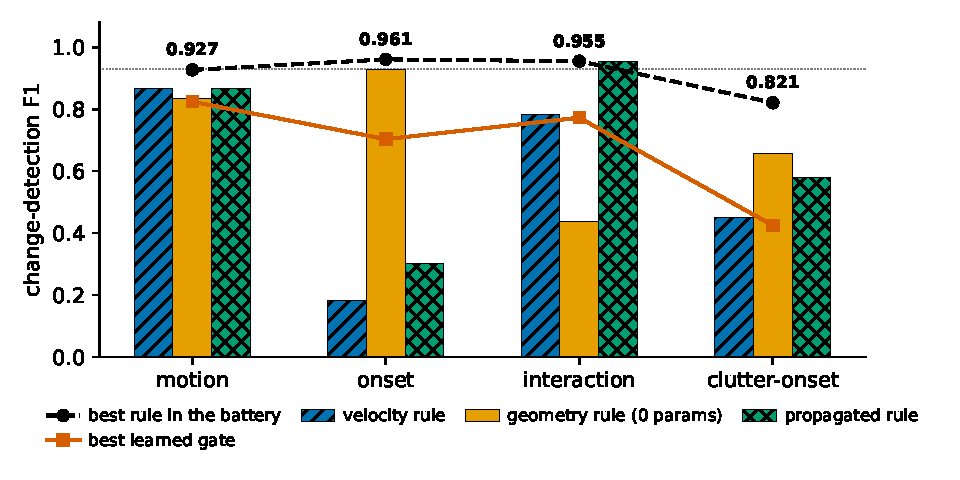
\includegraphics[width=0.92\textwidth]{figures/pattern}
\caption{Each filter removes its predecessor's shortcut and the ceiling does not move. Bars
are three rules from different groups of the battery; each collapses on the benchmark built
against it. The dashed line is the best of all eleven rules, which stays above $0.93$ on the
three filtered benchmarks and falls to $0.821$ only under dense packing; the solid line is the
best learned gate, which is below it everywhere and falls further.}
\label{fig:pattern}
\end{figure}

Table~\ref{tab:battery} and Figure~\ref{fig:pattern} contain the paper's central result. We
take the three benchmarks in the order they were built.

\paragraph{The motion benchmark is won by velocity.} The standard construction keeps steps in
which something moved. On it, \texttt{already\_moving}---predict change if and only if the
object is currently in motion---reaches F1 $0.866$, and the hand combination
\texttt{moving\_or\_near} reaches $0.927$, against the best learned gate's $0.824$. The reason
is immediate once measured: $P(\text{changed} \mid \text{already moving})$ is $0.87$--$0.95$ on
this split, because filtering for real motion and then asking what will move mostly asks about
\emph{continuation}, which requires no prediction at all.

\paragraph{The onset filter removes velocity, and proximity takes over.} The repair is to keep
only transitions in which a \emph{stationary} object starts moving, which can happen only
through contact. It works: \texttt{already\_moving} collapses from $0.866$ to $0.182$, and it
removes the shortcut from the training signal as well as from the metric, so models trained
here do improve at genuine onset prediction. But a geometric rule takes its place.
\texttt{pusher\_near} reaches $0.932$ and \texttt{nearest\_to\_pusher}---predict change for the
single object closest to the actuator, nothing fitted, \emph{zero} parameters---reaches
$0.928$, higher than the velocity rule ever managed on the benchmark it dominated. The best
learned gate reaches $0.703$.

Two controls close the obvious escape routes. The gate can see contact: the velocity-free
\texttt{contact} featurisation exposes signed contact distance directly, and that model still
reaches only $0.703$ against a parameter-free rule over the same quantity. And the one-feature
logistic regression reaches $0.919$, within $0.02$ of the best hand rule and $0.22$ above the
gate. A benchmark whose label is recoverable by a convex model with two parameters is telling
us about the task, not about anyone's optimiser.

\paragraph{The interaction filter removes proximity, and propagation takes over.} The third
benchmark keeps only transitions in which a stationary object starts moving \emph{while some
other object is closer to the actuator}---change that reached the object indirectly, through a
contact chain. Construction was verified on the built splits: every kept row contains an
indirect onset, the indirect mover sits at a median $0.143$\,m from the actuator against the
nearest object's $0.061$\,m, and the nearest object also moves in $92.8\%$ of rows, so these
are genuine chains. It works, too: \texttt{nearest\_to\_pusher} collapses from $0.928$ to
$0.437$ and the one-feature logistic from $0.919$ to $0.731$. (Those onset values are the
five-seed ones in Table~\ref{tab:battery}; the interaction column has three seeds, and the
matched three-seed comparison gives $0.925 \rightarrow 0.437$ and $0.916 \rightarrow 0.731$.)
And then
\texttt{moving\_or\_near\_mover}---flag anything already moving \emph{or} adjacent to something
already moving---reaches $0.955$ against the best learned gate's $0.772$.

This is the result the pre-registration was for. Had we tested only the rules the third filter
was designed to defeat, we would have reported a corrected benchmark.

\paragraph{The proximity degeneracy is not a property of one simulator.} Rebuilding the onset
benchmark on the quasi-static planar domain---a different engine with a different contact
model, and the domain where the \emph{velocity} shortcut had been strongest (F1 $0.990$ before
the onset filter, against the tabletop's $0.901$)---reproduces the pattern and sharpens it.
The velocity rule duly collapses to $0.085$--$0.243$, and \texttt{moving\_or\_near} then
reaches $0.983$, above the tabletop's $0.961$, against a gate trained on that benchmark at
$0.772$. The
onset filter removes the velocity shortcut in both domains and exposes the geometric one in
both.

\paragraph{Dense packing lowers the ceiling---and lowers the models further.} The mechanism in
Section~\ref{sec:mechanism} predicts that these shortcuts survive because a single actuator
makes contact spatially unambiguous. The direct test is to remove that unambiguity: pack the
objects until several are nearly equidistant from the actuator, \emph{and} apply the onset
filter, so that neither velocity nor ``which object is closest'' is decisive. We built exactly
that on the high-friction Chipmunk2D domain at its designed separation of $0.07$\,m.

It is expensive to build, for a reason that is itself diagnostic: in dense high-friction
clutter objects are mostly already touching and jostling, so a clean stationary-to-moving
transition is rare---onset transitions are $0.20\%$ of steps against the tabletop's $1.6\%$. Reaching
a trainable split takes $12{,}000$ episodes per cell (Appendix~\ref{app:provenance}).

This is the one manipulation in the study that moves the trivial ceiling. The best rule falls
to $0.821$, well below the $0.93$--$0.96$ of the other three benchmarks, and the
parameter-free proximity rule falls further, to $0.656$: packing does what the mechanism
predicts. It is also the manipulation that makes the learned models look worst. The gate
reaches $0.425$ and its velocity-free variant $0.338$, so the battery's margin \emph{widens} to
$0.396$---the largest in the paper. Removing the shortcut did not hand the task to the learned
model; it made the task harder for both, and harder for the model faster. This is the sharpest
statement of our thesis available to us: the problem is not that these benchmarks are too easy,
it is that difficulty and discriminativeness are being confused. A benchmark can be made harder
without getting any better at telling a world model from a line of code.

\paragraph{A second degeneracy: the filters make the class balance easier.} The
\texttt{always\_change} floor is $0.413$ and $0.387$ on the first two benchmarks but rises to
$0.673$ on the interaction benchmark, within $0.04$ of the \emph{learned} gate's $0.709$.
Filtering for harder events selects multi-change steps, so the positive rate rises and flagging
everything gets better. Any benchmark that filters for difficulty should report this number.

% =====================================================================================
\section{Five published models}
\label{sec:published}

\begin{table}[t]
\caption{Five published object-centric world models against one line of code, implemented from
their papers, trained with their native objectives, capacity-matched to $\sim$8.5--8.8k
parameters, on identical splits. Every model flags essentially every object
(recall $0.993$--$1.000$); the trivial velocity rule beats all five on the motion benchmark
at every object count. C-SWM has no decoder, so its change-detection numbers come from a probe
trained on frozen latents; its native ranking metrics are reported in the text instead.
\textbf{The five rows agreeing to three decimals is the result, not a transcription error}: once
recall is pinned at $1$, precision is the split's positive rate $p$ and F1 is therefore exactly
$2p/(1+p)$ for every model, regardless of architecture. The models differ from each other only
in pose accuracy (unchanged-object L2 $0.064$--$0.089$), never in which objects they flag.
Mean over object counts $\{3,5,8\}$; five seeds on the motion benchmark, and on the onset
benchmark five seeds at $N=3,5$ and three at $N=8$.}
\label{tab:published}
\centering
\small
\begin{tabular}{lrrrrrr}
\toprule
& \multicolumn{3}{c}{motion benchmark} & \multicolumn{3}{c}{onset benchmark} \\
\cmidrule(lr){2-4}\cmidrule(lr){5-7}
model & F1 & onset F1 & recall & F1 & onset F1 & recall \\
\midrule
\textbf{trivial: already moving} & \textbf{0.866} & \textbf{0.000} & \textbf{0.833} & \textbf{0.182} & \textbf{0.000} & \textbf{0.108} \\
\midrule
GNS / DPI-Net \citep{sanchezgonzalez2020gns,li2019dpinet} & 0.414 & 0.109 & 1.000 & 0.387 & 0.365 & 1.000 \\
C-SWM \citep{kipf2020cswm} & 0.413 & 0.109 & 0.999 & 0.387 & 0.365 & 1.000 \\
SlotFormer \citep{wu2023slotformer} & 0.414 & 0.109 & 1.000 & 0.387 & 0.365 & 1.000 \\
PETS \citep{chua2018pets} & 0.414 & 0.109 & 1.000 & 0.387 & 0.365 & 1.000 \\
NPS \citep{goyal2021nps} & 0.414 & 0.109 & 1.000 & 0.387 & 0.365 & 1.000 \\
\bottomrule
\end{tabular}

\end{table}

A reader may grant that the gate we audit against is weak. Table~\ref{tab:published} answers that objection
with five published models, each implemented from its paper rather than adapted from our
architecture, each trained with its own objective: GNS/DPI-Net
\citep{sanchezgonzalez2020gns,li2019dpinet} with three message-passing steps and explicit
geometric edge features; C-SWM \citep{kipf2020cswm} with a contrastive energy objective and no
decoder; SlotFormer \citep{wu2023slotformer}, the one baseline that could recover velocity by
differencing its history window; PETS \citep{chua2018pets}, an ensemble of heteroscedastic
Gaussians trained by NLL; and NPS \citep{goyal2021nps}, sparse learned rules applied one per
object per step.

\paragraph{One line of code beats all five, at every object count.} On the motion benchmark the
trivial velocity rule scores $0.901 / 0.862 / 0.836$ at $N = 3/5/8$ against the \emph{best}
published model's $0.542 / 0.397 / 0.303$. A paired bootstrap on the \emph{difference}---seeds
are paired by split, so the difference is what the claim is about---excludes zero at every
count: $-0.359$, $-0.465$ and $-0.533$, the last with a $95\%$ interval of
$[-0.561, -0.505]$.

\paragraph{Every published model is degenerate in the strong sense.} Recall runs from $0.993$
to $1.000$: they flag every object. They differ from one another only in pose accuracy
(unchanged-object L2 $0.064$--$0.089$), never in knowing which objects move. This is the
strongest form of our finding, because it is a property of ungated regression as a class rather
than of any rung we built.

\paragraph{Sparsity over rules is not sparsity over change.} NPS is the closest published
relative of the change-gate idea and was pre-registered as the load-bearing check on our
attribution: if sparse rule selection already supplied change detection, the gate would have no
claim. Its recall is exactly $1.000$, indistinguishable from the rest. Sparsity over
\emph{which rule transforms an object} is a different axis from sparsity over \emph{whether an
object is transformed}, and having the first does not give the second.

\paragraph{On the onset benchmark the ranking inverts, and the models still lose.} The trivial
velocity rule collapses ($0.866 \rightarrow 0.182$) while the published models more than triple
their onset F1 ($0.109 \rightarrow 0.365$), which is exactly what the onset filter was built to
do. It is tempting to stop there and call the benchmark corrected. The battery shows that all five are beaten on the onset benchmark too---by the proximity rules
of Section~\ref{sec:three}, and by a \emph{wider} margin than the velocity rule beats them on
the motion benchmark.

\paragraph{Two findings we did not predict.} PETS's ensemble disagreement is the standard
gate-free way to read change out of a probabilistic model, and it works on the motion benchmark
(AUC $0.757$). On the onset benchmark it falls to $0.532$, close to chance: ensemble
disagreement detects change only where change means continuation. And C-SWM's \emph{own}
metric moves the other way---Hits@1 rises $0.288 \rightarrow 0.882$ and MRR
$0.512 \rightarrow 0.918$ from the motion to the onset benchmark---while its change-detection
probe stays degenerate. A model can be good on its native objective and carry no information
about which objects will move.

% =====================================================================================
\section{Why it happens}
\label{sec:mechanism}

The degeneracy is not a bug in any filter. With a single point-like actuator and a minimum
separation between objects, contact is spatially unambiguous: at any step the actuator is near
at most one object, and that object is the one that moves. \texttt{nearest\_to\_pusher} is then
close to an oracle. Both shortcuts are symptoms of one fact---the label is recoverable from a
single scalar, speed or distance---and a filter only chooses which scalar. That is why the
sequence in Section~\ref{sec:three} terminates the way it does rather than converging.

The prediction this yields is testable, and we tested it. If spatial ambiguity is what the
shortcut feeds on, then packing the scene should erode it. Packing alone does erode it a
little: on a dense-packed variant of the motion benchmark \texttt{nearest\_to\_pusher} falls
$0.823 \rightarrow 0.784$ and \texttt{pusher\_near} $0.805 \rightarrow 0.776$, while
\texttt{moving\_or\_near} still leads the learned gate $0.906$ to $0.823$. Combining packing
with the onset filter---the clutter-onset column of Table~\ref{tab:battery}, and the most
adversarial construction available inside this task class---erodes it much further, to $0.821$
overall and $0.656$ for the parameter-free rule.

So the mechanism is confirmed in the direction it predicts, and the confirmation is not a
repair. The same construction that costs the rules $0.14$ costs the learned gate $0.28$. What
the analysis identifies is a property of the task that bounds \emph{everything} evaluated on
it, not a difficulty knob that a benchmark designer can turn until learned models win.

What would escape the mechanism is not more of the same knob, but a task in which \emph{which}
object changes is not determined by any single local quantity: multiple simultaneous actuators,
so proximity is
ambiguous; occluded or long-range coupling, so the responsible contact is not visible in the
geometry; or delayed effects, so the change does not coincide with the contact that caused it.
Each is a change of task rather than of filter. We think this is the honest reading of a
negative result: the repair is not a fourth construction of the same kind. We built one, aimed
squarely at the mechanism, and it moved the ceiling without closing the gap. Anyone building a
fifth should run the battery on it before claiming otherwise.

% =====================================================================================
\section{What survives}
\label{sec:survives}

Three properties of the change gate hold up against the battery and the published baselines.

\paragraph{Error suppression on unchanged objects.} With detection held fixed, a hard gate
keeps error out of the static majority in a way an ungated monolith does not, and the advantage
\emph{compounds} with object count. From $N=3$ to $N=20$ the monolith's error on objects that
did not move climbs monotonically, $0.271 \rightarrow 0.438$, while the gated model stays flat
at $\sim$$0.001$--$0.002$ because it copies them verbatim; the gap is monotone across all five
counts ($0.270 / 0.279 / 0.324 / 0.384 / 0.435$). This replicates in a second environment and
is matched by none of the five published baselines. We quote the \emph{difference} rather than
the ratio: the ratio's denominator is a near-zero false-positive rate that swings it by
$2\times$ between adjacent counts while meaning almost nothing.

\paragraph{The gate is usable as a local causal mask.} Used to generate counterfactual data by
relocating objects it marks unaffected \citep{pitis2020coda}, and checked against the simulator
by restoring an exact snapshot and perturbing only the objects under test, the learned gate
matches the ground-truth mask closely: the fraction of relocated objects that stay put, as the
synthetic label asserts, is $0.942$ for both at $N=3$ and within $0.014$ at every count, against
$0.865$ for causally blind relocation. The advantage over blind splicing grows with object
count ($+0.077 / +0.127 / +0.154$). The stricter test, which also requires every untouched object
to move exactly as in the real step, separates the gate slightly from the ground truth at higher
counts ($0.943 / 0.858 / 0.799$ against $0.946 / 0.906 / 0.839$) and both sharply from blind
relocation ($0.760 / 0.438 / 0.225$). Means over three seeds. Unlike the
error-suppression result this is not definitional: nothing about the architecture guarantees
that a gate trained for change detection produces placements a physics engine agrees with.

\paragraph{Velocity-free featurisation is what buys onset prediction.} Trained on the onset
benchmark, the \texttt{contact} featurisation beats the velocity-based one at every count, with
the margin widening in object count. The reciprocal check is worth stating because it explains
the first benchmark's failure: \texttt{contact} is \emph{worse} on already-moving objects, since
it cannot see velocity. The two featurisations solve different halves of the problem, and the
motion benchmark scored only the half that needs no prediction.

% =====================================================================================
\section{Limitations}
\label{sec:limitations}

\textbf{Task class.} Every claim here is bounded to single-actuator manipulation with local
contact. Section~\ref{sec:mechanism} states what falls outside it; we have not shown that
multi-actuator or long-range-coupling benchmarks are degenerate, and we predict they are not,
by the same argument.

\textbf{Privileged state, not pixels.} We audit models given object poses. Re-running the study
from $96\times96$ images is the natural next step, and it is blocked at perception for a reason
we can now quantify. Objects cover about $0.7\%$ of the frame, so a decoder reproducing the
background alone already attains most of the achievable reconstruction loss. Slot Attention
\citep{locatello2020slot} reaches a match distance of $25.8$\,px and a spatial-softmax keypoint
encoder \citep{finn2016spatial} $20.3$\,px, against a chance level of $\sim$$33$\,px and a
healthy one below $10$, on objects $8$\,px across. A foreground-weighted reconstruction loss
does not close the gap: it moves the keypoint encoder from $21.0$ to $20.3$\,px.

\textbf{Why we do not report the pixel comparison itself.} Those runs do produce
change-detection numbers, and taken at face value they point the other way: the learned
conditions beat the trivial pixel rule ($0.882$ vs.\ $0.703$), the reverse of every
state-space result here. We do not think that reading is available, and the arithmetic is the
reason. ``Changed'' is a displacement of $0.020$\,m, and at this resolution the world spans
$158$\,px per metre, so the label is defined by a \textbf{$3.2$\,px} shift --- while the front
end localises objects to within \emph{$20$\,px}. The trivial rule reads a centroid difference
and is therefore measuring noise six times larger than its signal; the learned conditions
consume the whole slot embedding and are not handicapped in the same way. The comparison is not
a test of the degeneracy, it is a test of the perception stack, and the perception stack fails
it. That the pixel study is single-seed and single-object-count only compounds it. The
privileged-state limitation therefore stands, and what these runs add is a sharper statement of
what would have to be fixed first.

\textbf{Seed counts and coverage.} The motion and onset columns use five seeds at each of
three object counts; the interaction and clutter-onset columns use three seeds at two object
counts, and both exclude $N=3$, where the filtered event is rare enough that a cell lands at or
below the $250$-train/$35$-test floor we hold everything else to. Seed counts this small put a floor
under the $p$-value itself: an exact paired sign-flip test on $n$ seeds has $2^n$ outcomes, so
the smallest attainable $p$ is $0.250$ at $n=3$ and $0.0625$ at $n=5$. Every published-model
comparison in Section~\ref{sec:published} sits exactly at the $n=5$ floor, which means the
seeds agree unanimously and \emph{not} that the effect is marginal --- a $p$ at its floor is
uninformative about effect size in either direction. We therefore quote bootstrap intervals on
the paired difference throughout, and treat significance claims as unavailable at these seed
counts.

\textbf{Control.} We do not claim the gate helps control. In a CEM
\citep{rubinstein2004cem} comparison over three training seeds and $20$ held-out episodes each,
where the scripted oracle reaches $1.000$ (so the planner and cost are sound and every deficit
is model quality), PETS is the strongest published planner at every seed ($0.267$ pooled) and
NPS the only other one above zero at every seed ($0.133$); GNS and C-SWM ($0.083$ each) and
SlotFormer ($0.033$) plan at some seeds and not others. Our model reaches $0.250$ pooled over the
same three seeds and episodes, which is not distinguishable from PETS, since a success rate over
$20$ episodes carries roughly $\pm 0.10$. Single-seed planning comparisons are unreliable here:
our own model scores $0.150$ at one seed and $0.300$ at the other two.

% =====================================================================================
\section{Conclusion}

Change detection is the capability object-centric world models are most often credited with,
and on current benchmarks it is not measured. Three successive benchmarks, each built to remove
the last one's shortcut, are each won by a rule with at most one parameter; five published
models lose to those rules everywhere and flag essentially every object as changing. A fourth,
aimed at the mechanism rather than the symptom, lowers the trivial ceiling for the first time
and lowers the learned models further---which is the clearest evidence we have that difficulty
and discriminativeness are separate axes, and that this literature has been tuning the wrong
one. The mechanism is structural, so the repair is a different task rather than a better
filter. We release the battery, and we suggest the requirement it implies: report the best
trivial rule next to the model, and invent the rules against the benchmark being proposed
rather than the one it replaces.

% =====================================================================================
\section*{Reproducibility statement}
Every number in this paper is emitted from a run directory by
\texttt{experiments/make\_iclr\_tables.py}, which writes the tables and figure the manuscript
\texttt{\textbackslash input}s; a stage that has not run appears as \texttt{--} rather than
being silently omitted, and Appendix~\ref{app:provenance} lists the cell count behind every
column. The \texttt{config.json} and \texttt{summary.json} of every run are included in the
supplementary material, so each table cell can be traced to the configuration that produced it
without rerunning anything. The analysis ledger in \texttt{experiments/RESULTS.md} records the
provenance of every claim, and \texttt{paper/claims.py} recomputes every number in the paper
from the run artifacts. Data generation is seeded, and the pipeline scripts named in the ledger
regenerate every run from scratch: rule scores and simulator statistics reproduce exactly, and
retrained models to within the seed-to-seed variation we report. Splits are episode-disjoint via
\texttt{experiments/build\_clean\_splits.py}. The audit battery runs on any benchmark via
\texttt{python -m experiments.audit\_battery --test yours\_test.npz --val yours\_val.npz}. The
test suite pins metrics, splits and the browser export. An interactive demonstration that runs
the trained gate against live physics in a browser, and scores it against the battery frame by
frame, is included in the anonymised supplementary material.

% =====================================================================================
\section*{Use of large language models}
An AI coding assistant was used to implement methods, design and iterate on
experiments, clean and reformat datasets, and interpret results. Specifically:
the audit battery, the four-engine domain suite, the five literature baselines
(GNS/DPI-Net, C-SWM, SlotFormer, PETS, NPS), the sparse and dense models, and the
browser demonstration were implemented with assistance; the contact featurisation,
the experiment analysis, and the drafting of this manuscript were iterated with its
feedback. All claims, numbers, and statistical tests were verified by the authors
against the run artifacts and the analysis ledger; the authors remain responsible for
every claim and for any error the assistant may have introduced.

\bibliographystyle{iclr2027_conference}
\bibliography{iclr2027_conference}

\appendix
\section{Provenance of every column}
\label{app:provenance}
The audit is only as strong as its coverage, so we state it rather than summarising it. Each
column of Table~\ref{tab:battery} rests on the following runs and cells, emitted alongside the
table by the same script.

\begin{center}
\small
\begin{tabular}{llrl}
\toprule
benchmark & run directory & cells & seeds $\times$ object counts \\
\midrule
motion & \texttt{onset\_shortcut\_audit\_5seed} & 15 & seeds 0,1,2,3,4 $\times$ N=3,5,8 \\
onset & \texttt{onset\_shortcut\_audit\_5seed} & 15 & seeds 0,1,2,3,4 $\times$ N=3,5,8 \\
interaction & \texttt{audit\_interaction\_billiards} & 6 & seeds 0,1,2 $\times$ N=5,8 \\
clutter-onset & \texttt{audit\_onset\_clutter12k} & 6 & seeds 0,1,2 $\times$ N=5,8 \\
\bottomrule
\end{tabular}

\end{center}

\paragraph{Split sizes.} Rows per cell after filtering, which is the quantity that decides
whether a cell can be trained on at all: the motion and onset benchmarks sit near
$750$--$950$ training rows, and the clutter-onset benchmark at $12{,}000$ episodes per cell
reaches $697$--$1225$ training and $81$--$156$ test rows. We hold every cell to a floor of
$250$ training and $35$ test rows; no reported cell falls below it. Two constructions were
excluded on this ground rather than quietly included: $N=3$ for the interaction benchmark, and
$N=3$ for clutter-onset, which would need roughly $27{,}000$ episodes per cell to clear the
floor. Below that floor a learned model's score is as likely to reflect data starvation as
anything about the benchmark.

\section{The full battery}
\label{app:battery}
Table~\ref{tab:battery} shows the rules the argument turns on. For completeness, here is every
rule the battery scores, on every benchmark, grouped as in Section~\ref{sec:battery}. The
fitted radii and the rule definitions are emitted alongside these numbers by the audit script.

Two things are visible here that the main table has no room for. First, the geometric group
degrades gracefully rather than collapsing: \texttt{pusher\_approaching} and
\texttt{two\_nearest\_to\_pusher} hold $0.66$--$0.73$ almost everywhere, so a benchmark that
defeats one geometric rule has usually not defeated the family. Second,
\texttt{second\_nearest\_to\_pusher} is the only rule that is bad on every benchmark
($0.10$--$0.41$), which is the sanity check on the battery: a proximity rule pointed at the
wrong object should fail, and it does.

\begin{center}
\small
\begin{tabular}{llrrrr}
\toprule
rule & group & motion & onset & interaction & clutter-onset \\
\midrule
\texttt{already\_moving} & kinematic & 0.866 & 0.182 & 0.783 & 0.449 \\
\midrule
\texttt{nearest\_to\_pusher} & geometric & 0.836 & 0.928 & 0.437 & 0.656 \\
\texttt{pusher\_approaching} & geometric & 0.529 & 0.691 & 0.729 & 0.683 \\
\texttt{pusher\_near} & geometric & 0.812 & 0.932 & 0.715 & 0.698 \\
\texttt{second\_nearest\_to\_pusher} & geometric & 0.163 & 0.095 & 0.405 & 0.219 \\
\texttt{two\_nearest\_to\_pusher} & geometric & 0.692 & 0.698 & 0.679 & 0.656 \\
\midrule
\texttt{moving\_or\_near\_mover} & propagated & 0.866 & 0.302 & 0.955 & 0.579 \\
\texttt{near\_a\_mover} & propagated & 0.263 & 0.210 & 0.712 & 0.441 \\
\texttt{near\_pusher\_or\_mover} & propagated & 0.831 & 0.935 & 0.820 & 0.782 \\
\midrule
\texttt{moving\_or\_near} & combination & 0.927 & 0.961 & 0.858 & 0.821 \\
\midrule
\texttt{always\_change} & floor & 0.413 & 0.387 & 0.673 & 0.485 \\
\midrule
\texttt{logistic\_on\_distance} & control & 0.810 & 0.919 & 0.731 & 0.577 \\
\midrule
learned gate (velocity features) & learned & 0.824 & 0.508 & 0.709 & 0.425 \\
learned gate (velocity-free) & learned & 0.688 & 0.703 & 0.772 & 0.338 \\
\bottomrule
\end{tabular}

\end{center}

\section{Per-domain characterisation}
\label{app:domains}
The precondition for the velocity shortcut is measured directly on the simulators, with no model
trained: three object counts $\times$ three seeds $\times$ $60$ episodes per domain, produced by
\texttt{experiments/domain\_characterization.py}. The motion threshold for each domain is derived
as described in Section~\ref{sec:setup}.

\begin{center}
\small
\begin{tabular}{lllrrrrr}
\toprule
domain & engine & contact regime & $P(\text{chg}\mid\text{moving})$ & $P(\text{chg}\mid\text{rest})$
& ratio & changed frac. & threshold \\
\midrule
\texttt{billiards} & Box2D & near-elastic & $0.982$ & $0.020$ & $50\times$ & $0.394$ & $0.031$ \\
\texttt{planar} & ours & quasi-static & $0.950$ & $0.011$ & $84\times$ & $0.152$ & $0.010$ \\
\texttt{clutter} & Chipmunk2D & high-friction, packed & $0.863$ & $0.024$ & $36\times$ & $0.345$ & $0.028^{*}$ \\
\texttt{tabletop} & MuJoCo & impulsive 3D & $0.714$ & $0.015$ & $48\times$ & $0.124$ & $0.020$ \\
\bottomrule
\end{tabular}

\smallskip
\footnotesize $^{*}$The clutter benchmarks are built with a threshold of $0.029$.
\end{center}

The shortcut exists in every domain. It is strongest under near-elastic contact (billiards,
$0.982$), where objects keep moving after a hit, and weakest on the MuJoCo tabletop ($0.714$),
whose 3D solver lets a box come to rest through tilting and settling that a 2D engine cannot
represent, so more of its moving objects stop within one step.

The threshold derivation has two self-checks. It returns $0.020$ for the tabletop, the value it
was anchored to, and $0.010$ for planar, the value that domain independently requires. The
anchor is the fraction of steps retained rather than a statistic of moved-object displacement,
since the latter is measured on an already-filtered split and would make the derivation
circular.

\end{document}
